\documentclass[a4paper, 11pt]{article}
\usepackage[utf8]{inputenc}
\usepackage{mathtools}
\usepackage{amsmath}
\usepackage{titlesec}
\usepackage{amssymb}
\usepackage{gensymb}
\usepackage[catalan]{babel}
\usepackage[dvipsnames]{xcolor}
\usepackage[margin=1in]{geometry}
\usepackage[hidelinks]{hyperref}
\usepackage{fancyhdr}
\usepackage{graphicx}
\usepackage{cancel}
\usepackage{subcaption}
\usepackage{tabto}
\usepackage{subcaption}
\usepackage{tocloft}
\usepackage{float}
\usepackage[style=numeric-comp, sorting=none]{biblatex}
\bibliography{bib.bib}
\newcommand{\figuretag}[1]{%
  \addtocounter{figure}{-1}%
  \renewcommand{\thefigure}{#1}%
}


\setcounter{tocdepth}{1}
\renewcommand{\cftdot}{.}
\pagestyle{fancy}
\lhead{Treball de Simulació}
\rhead{}

\begin{document}
\begin{figure}
    \centering
    
\includegraphics[width=0.6\textwidth]{images/Logo_uab.png}
   % \caption{Caption}%
    \label{uab}
\end{figure}

\title{{\textbf{\Large LLIURAMENT D'INTRODUCCIÓ A L'ASTROFÍSICA: UNDERSTANDING ANALEMMAS
}\\}

\vspace{12mm}

{\large Facultat de ciències}\\
{\large Introducció a l'Astrofísica}}

\author{\textbf{Reina Delgado, Airan (1670808)}}
\date{}


\maketitle

\vspace{30mm} \title{\textbf{\Large ABSTRACT}}


%%%%%%%%%%%%%%%%%%%%%%%%%%%%%%%%%%%
%%%%%%%%%%%%%%%%%%%%%%%%%%%%%%%%%%%

    \vspace{4mm} 
    \noindent AGajkdkl
    \newpage

%%%%%%%%%%%%%%%%%%%%%%%%%%%%%%%%%%%
%%%%%%%%%%%%%%%%%%%%%%%%%%%%%%%%%%%
%%%%%%%%%%%%%%%%%%%%%%%%%%%%%%%%%%%
%%%%%%%%%%%%%%%%%%%%%%%%%%%%%%%%%%%
%%%%%%%%%%%%%%%%%%%%%%%%%%%%%%%%%%%

\section*{EXERCICI 1}
\noindent Un analema és la corba que descriu el Sol al cel si s’observa des d'un lloc fix, a la mateixa hora del dia, cada dia de l’any. L’analema forma una corba que, aproximadament sol ser, una forma de vuit o lemniscata. Es poden observar analemes en altres planetes del Sistema Solar, però tenen una forma diferent de la que s’observa a la Terra, podent arribar a ser corbes diferents d’un vuit (a Mart és molt semblant a una gota d’aigua), tot i que tenen com a característica comuna que sempre són tancades \cite{DEFINICIO_ANALEMA}. Un exemple d’analema és el que es pot observar a la figura \ref{fig:analema}.

\begin{figure}[h!]
    \centering
    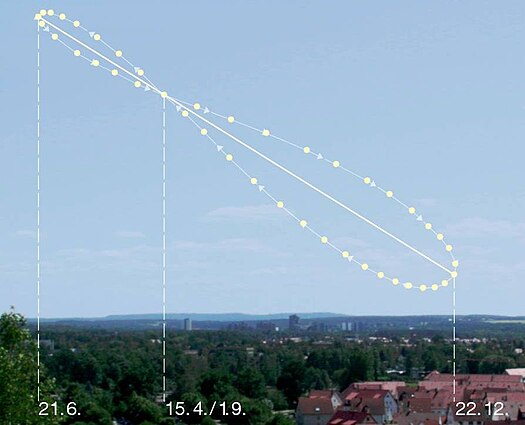
\includegraphics[width=0.6\textwidth]{images/analema.png}
    \caption{Analema solar per un observador a l'hemisfèri nord. Font: Wikipedia \cite{DEFINICIO_ANALEMA}.}
    \label{fig:analema}
\end{figure}


%%%%%%%%%%%%%%%%%%%%%%%%%%%%%%%%%%%
%%%%%%%%%%%%%%%%%%%%%%%%%%%%%%%%%%%

\section*{EXERCICI 2}
\noindent  En coordenades equatorials, un objecte en la bòveda celeste es pot localitzar amb les coordenades "ascensió recta" ($\alpha$ o $ra$) i "declinació" ($\delta$ o $dec$). El pla des d'ón es defineixen les coordenades és l'equador celestial, que és el pla perpendicular a l'eix de rotació de la Terra coincident amb l'equador terrestre. La declinació és l'angle entre l'equador i el cos celeste i, l'ascensió recta, és l'angle (En hores) del cos al voltant de l'equador celestial. El moviment vertical aparent del Sol en l'analema prové del canvi en la declinació solar al llarg de l'any degut a que la Terra orbita al voltant del Sol amb l'eix de rotació inclinat uns 23.5 graus respecte al pla de l'òrbita \cite{ANALEMA_WIKI}.
\vspace{5mm}

%%%%%%%%%%%%%%%%%%%%%%%%%%%%%%%%%%%
%%%%%%%%%%%%%%%%%%%%%%%%%%%%%%%%%%%

\section*{EXERCICI 3}
\noindent El moviment transversal (Est-Oest) aparent del Sol en l'analema prové del canvi no uniforme de l'ascensió recta solar al llarg de l'any degut als efectes combinats de la inclinació de l'eix de rotació de la Terra i l'eccentricitat de l'òrbita terrestre (Que genera una variació de la velocitat orbital de la Terra al llarg de l'any) \cite{ANALEMA_WIKI}. Aquests dos efectes generen una desigualtat en el moviment aparent del Sol al llarg de l’equador celeste, de manera que el Sol no arriba cada dia al meridià a la mateixa hora segons un rellotge mitjà. Aquest desfasament es quantifica mitjançant l’equació del temps, que expressa la diferència entre el temps solar veritable (Marcat per la posició real del Sol) i el temps solar mitjà (Definit per un moviment solar fictici uniforme) \cite{EQ_OF_TIME}.
\vspace{5mm}

%%%%%%%%%%%%%%%%%%%%%%%%%%%%%%%%%%%
%%%%%%%%%%%%%%%%%%%%%%%%%%%%%%%%%%%

\section*{EXERCICI 4}
\noindent 
\vspace{5mm}

%%%%%%%%%%%%%%%%%%%%%%%%%%%%%%%%%%%
%%%%%%%%%%%%%%%%%%%%%%%%%%%%%%%%%%%

\section*{EXERCICI 5}
\noindent ahajaklsl
\vspace{5mm}

%%%%%%%%%%%%%%%%%%%%%%%%%%%%%%%%%%%
%%%%%%%%%%%%%%%%%%%%%%%%%%%%%%%%%%%

\section*{EXERCICI 6}
\noindent ahajaklsl
\vspace{5mm}

%%%%%%%%%%%%%%%%%%%%%%%%%%%%%%%%%%%
%%%%%%%%%%%%%%%%%%%%%%%%%%%%%%%%%%%

\section*{EXERCICI 7}
\noindent ahajaklsl
\vspace{5mm}

%%%%%%%%%%%%%%%%%%%%%%%%%%%%%%%%%%%
%%%%%%%%%%%%%%%%%%%%%%%%%%%%%%%%%%%

\section*{EXERCICI 8}
\noindent ahajaklsl
\vspace{5mm}

%%%%%%%%%%%%%%%%%%%%%%%%%%%%%%%%%%%
%%%%%%%%%%%%%%%%%%%%%%%%%%%%%%%%%%%

\section*{EXERCICI 9}
\noindent ahajaklsl
\vspace{5mm}

%%%%%%%%%%%%%%%%%%%%%%%%%%%%%%%%%%%
%%%%%%%%%%%%%%%%%%%%%%%%%%%%%%%%%%%

\section*{EXERCICI 10}
\noindent ahajaklsl
\vspace{5mm}

%%%%%%%%%%%%%%%%%%%%%%%%%%%%%%%%%%%
%%%%%%%%%%%%%%%%%%%%%%%%%%%%%%%%%%%
























%%%%%%%%%%%%%%%%%%%%%%%%%%%%%%%%%%%
%%%%%%%%%%%%%%%%%%%%%%%%%%%%%%%%%%%
%%%%%%%%%%%%%%%%%%%%%%%%%%%%%%%%%%%
%%%%%%%%%%%%%%%%%%%%%%%%%%%%%%%%%%%
%%%%%%%%%%%%%%%%%%%%%%%%%%%%%%%%%%%

\newpage
\printbibliography
\end{document}